
\section{Design}

\begin{figure*}
\centering
%\includegraphcs[width=1.0\columnwidth]{system.pdf}
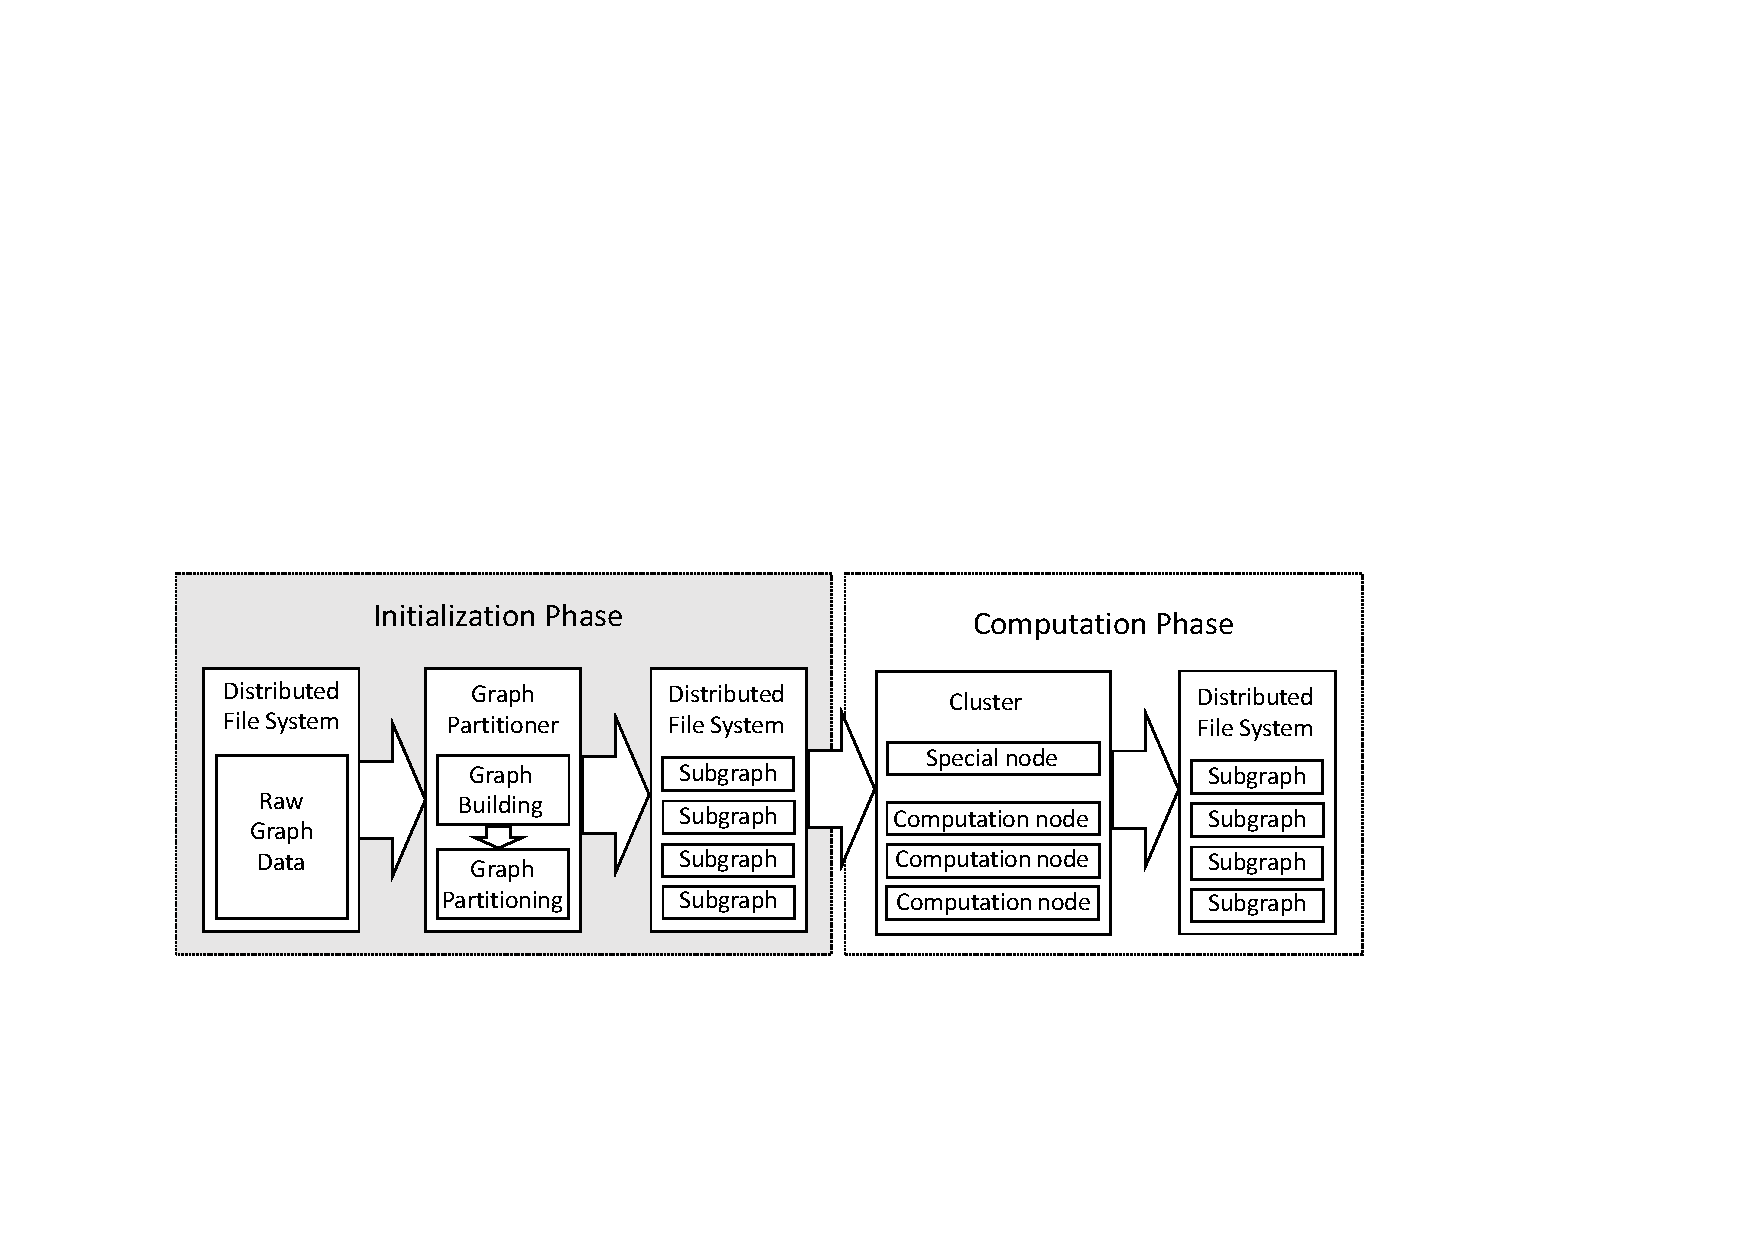
\psfig{file=system.pdf, height=2in, width=6.5in}
\caption{A high level overview of the system}
%\tightcaption{aaaa}
\label{fig:cdn}
\end{figure*}

\subsection{Distributed data graph}
Efficiently partitioning the data graph in the distributed environment requires balancing computation, communication, and storage. 
Therefore, we need to construct balanced subgraphs that minimize number of edges/nodes that cross between machines. 

PowerGraph achieves balanced partitioning by considering the strongest feature of natural graphs: having highly skewed power-law degree distributions.~\cite{powerGraph} 
We used the same partitioning strategy and stored each part as a separate file on a distributed storage system (e.g., HDFS, Amazon S3).

\subsection{Configuration management}
The system needs management during the computation. 
At initialization phase, the graph is torn down to several atom graphs and mapped to each machines. 
Machines are assigned by ZooKeeper. A subset of nodes are assigned to particular tasks (e.g., shared data table), while the remaing nodes are assigned to do the computation. 
Some idle nodes remains in a pool which can be used as needed (e.g., a node might registered as a stanby for multiple active nodes). 

ZooKeeper maintains overall system status and stays reliable when the fault occurs. Thus, the system would remain safe over the fault management by ZooKeeper.

%\subsection{
\subsection{Scheduler}
The scheduler represents a dynamic list of tasks to be executed. Since new messages are calculated from the previous incoming messages, if a message is updated, the messages on the connected edges need update as well. 

The schedule management is also designed with ZooKeeper. ZooKeeper maintains consistency between parallel updates with distributed locks. 
The computation iterates until convergence. ZooKeeper terminates the computation from all the nodes when the system reaches convergence. 


\subsection{System design}
In Fig. 1, we provide a high-level overview of the system. 
The computation begins by constructing subgraph representation on a Distributed File System (DFS). 
%Fig. provides the high-level overview of the computation engine. 

Each instance is executed on each machine. 
Some nodes are assigned to particular tasks and the rest of them are assigned to computation. 
